\documentclass[a4paper,12pt]{report}

\usepackage[utf8]{inputenc}
\usepackage[frenchb]{babel}
\usepackage[T1]{fontenc}
\usepackage{lmodern}
\usepackage{layout}
\usepackage[top=2cm, bottom=2cm, left=3cm, right=2cm]{geometry}
\usepackage{setspace}
\usepackage{verbatim}
\usepackage{moreverb}
\usepackage{listings}
\usepackage{graphicx}
\usepackage{shorttoc}
\usepackage[nonumberlist]{glossaries}
\usepackage{xcolor}

% Têtes de chapitre
\usepackage{xcolor}
%\usepackage{biblatex} 

% Tête de chapitre
\makeatletter
\newlength{\chapter@number@width}
\def\@makechapterhead#1{%
  {\normalfont
  \setlength{\parindent}{0pt}%
  \vspace*{10pt}%
  \settowidth{\chapter@number@width}{%
    \hbox{\color{white}\LARGE\bfseries
          \hspace{\dimexpr 1mm+3pt}%
          \thechapter
          \hspace{\dimexpr 1mm+3pt}%
    }}
  \hbox{%
    \vtop{%
      \hsize=\dimexpr\chapter@number@width+\tabcolsep+2\fboxrule+\tabcolsep
      \begin{tabular}[t]{@{}c}
        \scshape\strut\makebox[0pt]{\hspace{0pt plus 1 fill minus 1 fill}\@chapapp\hspace{0pt plus 1 fill minus 1 fill}} \\
        \fboxsep=0pt
        \colorbox{black}{\vbox{%
           \hbox{\vbox to \dimexpr 1mm+3pt{}}
           \hbox{\color{white}\LARGE\bfseries
                 \hspace{\dimexpr 1mm+3pt}%
                 \thechapter
                 \hspace{\dimexpr 1mm+3pt}%
                }
           \hrule height 0.4pt depth 0pt width 0pt
           \hbox{\vbox to 6pt{}}
           \hbox{\parbox{0pt}{\Huge\bfseries\vphantom{E}}}
           }}%
      \end{tabular}%
      }%
    \vtop{%
      \advance\hsize by -\dimexpr\chapter@number@width+2\fboxrule+\tabcolsep
      \hspace*{-0.5cm}\begin{tabular}[t]{c}
        \scshape\strut\vphantom{\@chapapp} \\
        \fboxsep=0pt
        \colorbox{white}{\vbox{%
           \hbox{\vbox to \dimexpr 1mm+3pt{}}
           \hbox{\LARGE\bfseries
                 \hspace{\dimexpr 1mm+3pt}%
                 \phantom{\thechapter}
                 \hspace{\dimexpr 1mm+3pt}%
                }
           \hrule height 0.4pt depth 0pt width \hsize
           \hbox{\vbox to 6pt{}}
           \hbox{\hspace*{20pt}\parbox{\dimexpr\textwidth-2mm-6pt-\chapter@number@width-\tabcolsep-2\fboxrule-20pt}{\Huge\bfseries #1}}
           }}%
      \end{tabular}%
      }%
    }%
  \vspace{50pt}%
  }
}
\def\@makeschapterhead#1{%
  {\normalfont
  \setlength{\parindent}{0pt}%
  \vspace*{10pt}%
  \settowidth{\chapter@number@width}{%
    \hbox{\color{white}\LARGE\bfseries
          \hspace{\dimexpr 1mm+3pt}%
          \thechapter
          \hspace{\dimexpr 1mm+3pt}%
    }}
  \hbox{%
    \vtop{%
      \hsize=\dimexpr\chapter@number@width+\tabcolsep+2\fboxrule+\tabcolsep
      \begin{tabular}[t]{@{}c}
        \scshape\strut\makebox[0pt]{\hspace{0pt plus 1 fill minus 1 fill}\phantom{\@chapapp}\hspace{0pt plus 1 fill minus 1 fill}} \\
        \fboxsep=0pt
        \colorbox{black}{\vbox{%
           \hbox{\vbox to \dimexpr 1mm+3pt{}}
           \hbox{\color{white}\LARGE\bfseries
                 \hspace{\dimexpr 1mm+3pt}%
                 \phantom{\thechapter}%
                 \hspace{\dimexpr 1mm+3pt}%
                }
           \hrule height 0.4pt depth 0pt width 0pt
           \hbox{\vbox to 6pt{}}
           \hbox{\parbox{0pt}{\Huge\bfseries\vphantom{E}}}
           }}%
      \end{tabular}%
      }%
    \vtop{%
      \advance\hsize by -\dimexpr\chapter@number@width+2\fboxrule+\tabcolsep
      \hspace*{-0.5cm}\begin{tabular}[t]{c}
        \scshape\strut\vphantom{\@chapapp} \\
        \fboxsep=0pt
        \colorbox{white}{\vbox{%
           \hbox{\vbox to \dimexpr 1mm+3pt{}}
           \hbox{\LARGE\bfseries
                 \hspace{\dimexpr 1mm+3pt}%
                 \phantom{\thechapter}
                 \hspace{\dimexpr 1mm+3pt}%
                }
           \hrule height 0.4pt depth 0pt width \hsize
           \hbox{\vbox to 6pt{}}
           \hbox{\hspace*{20pt}\parbox{\dimexpr\textwidth-2mm-6pt-\chapter@number@width-\tabcolsep-2\fboxrule-20pt}{\Huge\bfseries #1}}
           }}%
      \end{tabular}%
      }%
    }%
  \vspace{50pt}%
  }
}
\makeatother

% Verbatim langage
%\lstset{
%	language=Python,
%	basicstyle=\footnotesize,
%	basicstyle=\ttfamily\small,
%	keywordstyle=\color{blue}\bfseries\emph,
%	stringstyle=\color{black!60},
%	columns=flexible,
%	tabsize=4,
%	extendedchars=true,
%	showspaces=false,
%	showstringspaces=false,
%	breaklines=true,
%	breakautoindent=true,
%	captionpos=b,
%	numbers=left,
%	numberstyle=\footnotesize,
%	stepnumber=1,
%	numbersep=10pt,
%	frame=single
%}


% Redéfinition de commandes
\renewcommand{\baselinestretch}{1.5}
\renewcommand\thesection{\arabic{section}}
\renewcommand\thesection{\arabic{chapter}.\arabic{section}}

% Définition de commandes
%\newcommand{\EX}{\emph{Exemple}}

%Mots sans césures
%\hyphenation{Exemple} 

% Désactiver les alinéas automatiques
\parindent = 0pt

% Elements pour la page de garde
\title{Titre}
\author{Philippe Chauvelin}
\date{\today}

% Création du glossaire
\makeglossaries
%\newglossaryentry{erp}{
%	name={ERP },
%	text={ERP*},
%	description={\textbf{(Enterprise Resource Planning) :} Progiciel permettant de gérer l'ensemble des processus d'une entreprise en intégrant l'ensemble de 
%	ses fonctions comme la gestion des ressources humaines, la gestion financière et comptable, l'aide a la décision, la vente, la distribution 
%	l'approvisionnement, la production ou encore du e-commerce. Parfois appelé \textbf{PGI (Progiciel de Gestion Intégré)} avec la dénomination française}
%}
%
%\newglossaryentry{opensource}{
%	name={OPEN SOURCE :},
%	text={Open Source*},
%	description={Logiciels dont la licence respecte les critères définis par l'association Open Source Initiative (OSI). Parmi ces critères, on retrouve 
%	la possibilité de libre redistribution, d'accès au code source et de Travaux dérivés}
%}

% Début du document	
\begin{document}
	% Page de garde 
	\begin{titlepage}
		\begin{center}
			Philippe CHAUVELIN - François-Guillaume RIBREAU\\
			CSII 3\ieme~année\\
		\end{center}
		\hrulefill
		\vspace{7cm}
		\begin{center} 
			\LARGE \textbf{Les attaques XSS}\\
			\vspace{6cm}
		
			\begin{tabular}{cp{4cm}c}
				
\includegraphics[height=75px]{images/logo_epsi.jpg}\\
				\textbf{E.P.S.I - NANTES}\\
				114 rue des Hauts Pavés\\
				BP 41903\\
				44019 NANTES CEDEX 01\\
			\end{tabular}
		\end{center}
	\end{titlepage}
	\newpage
	
	% Page vierge
	\newpage
	\null
	% Met le compteur de numérotation à zéro et n'affiche pas le numéro de page remerciement
	\thispagestyle{empty}
	\setcounter{page}{0}
	\newpage
	
	
	% Sommaire
	\shorttableofcontents{Sommaire}{0}
	\setcounter{page}{1}
	\thispagestyle{empty}
	\newpage
	
	% Introduction
	\chapter*{Introduction} % (fold)
		% Ajout de Introduction dans le sommaire mais sans numéro		
		\setcounter{section}{1}
		
		\addcontentsline{toc}{chapter}{Introduction}
		
« Au printemps dernier, les dirigeants de Sony présentent leurs excuses à 75 millions d'utilisateurs pour ne pas avoir suffisamment protégé leurs comptes. ».\\

Sony est une multinationale japonaise spécialisée dans le domaine du multimédia. Au printemps dernier, celle-ci à mis plus d'une semaine avant de remarquer qu'elle se faisait voler les données personnelles de près de 75 millions de joueurs abonnés à son réseau Playstation Network. Une erreur qui lui coutera environ 171 millions de dollars. Symantec, créateur de la suite de sécurité Norton, estime les pertes infligées par la cybercriminalité à près de 271 milliards d'euros, et le nombre de cybercrime quotidien à un million.\\

L’expansion de l’informatique conduit de plus en plus de personnes à développer leurs propres programmes, que ça soit pour une entreprise ou pour une utilisation personnelle. Cette expansion est une porte ouverte au piratage, de plus en plus courant en raison du nombre de développeurs qui augmente chaque année. Les Exploits, faisant partie de nos jours des logiciels malveillants les plus utilisés par les pirates, sont de plus en plus virulents.
Ce thème est très intéressant car il nous permettra de nous pencher sur l'une des failles les plus courantes du moment. \textbf{Nous allons donc dans ce rapport aborder les différents vecteurs d'attaque et de protection des applications Web relatives aux failles XSS}.\\

Une faille XSS est un Exploit visant à injecter du code (généralement Javascript) malveillant dans une page d'un site qui sera exécuté par le navigateur de la victime. Elle à pour but la récupération d'informations personnelles sur cette dernière afin de permettre l'usurpation d'identité (phishing) ou alors la propagation d'un virus comme par exemple le virus Samy qui a  contaminé plus de un million de profils MySpace. \\

Nous aborderons dans une première partie le fonctionnement détaillé d'une faille XSS , et plus particulièrement la phase de détection de celle-ci. La résultante de cette dernière nous amènera à conclure l'existence de deux sous-catégories de cette famille de faille. La première sous-catégorie et la moins dangereuse est le XSS réfléchi. Elle permet, via l'injection de code Javascript dans une url menant à un site non protégé, de contrôler le contenu de celui-ci. Elle est considérée comme moins par la communauté des développeurs étant donné qu'il est presque nécessaire d'utiliser l'ingénierie sociale pour assurer son fonctionnement. D'un autre coté, on distinguera le XSS stocké, ou permanent. Cette faille est à l'origine des plus grandes attaques XSS de l'histoire du Web (MySpace, Twitter, etc.). Contrairement au XSS réfléchi, le code injecter peut être stocké sur le serveur et par conséquent toucher un grand nombre de personnes (Exemple : injection de code malveillant dans un forum non protégé). La compréhension de ces différents éléments nous permettra d'aborder les solutions envisageables afin de protéger ses applications Web telles que la protection des ajouts en base de données, la protection des cookies disposant d'informations sur l'utilisateur ou encore les différentes solutions proposés par les langages et Framework.  \\

« Les entreprises investissent d'avantage dans leurs machines à café que dans la sécurité informatique ».\\

Yahoo, le 12 février 2006, contracte un ver XSS nommé Yammaner, basé sur  Samy de MySpace et ayant pour but de voler la liste de contact de la victime. Pour cela cette dernière recevait un email qui une fois ouvert s’envoyait lui-même à tous les contacts de la victime.


		
			
		% chapter Introduction (end)
		\newpage
	
	% Chapitre 1
	\chapter{Approche théorique} % (fold)
	% Section 1	
	\section{Définition}	
Le XSS est une attaque visant les sites web qui affichent dynamiquement du contenu côté client et ce sans effectuer de contrôle des informations saisies par les utilisateurs. Les exploits Cross-Site Scripting consistent à forcer un site web à afficher du code HTML ou des scripts non autorisés et saisis par les utilisateurs. Le XSS est donc une attaque menée dans le but d'exécuter un code Javascript directement sur le poste de la victime. Cette technique est particulièrement utilisée par les pirates pour voler la session d'un utilisateur connecté.
Si le pirate arrive à identifier un site web vulnérable, il a donc la possibilité d’insérer un script au sein d’une URL et de l’envoyé à une victime. Si cette dernière est connectée sur ce site web vulnérable, elle enverra immédiatement, et à son insu, son cookie de session au pirate. L'attaquant pourra alors utiliser ce cookie et voler la session de la victime pour mener des actions frauduleuses.

		

		\newpage
	

	\section{Recherche de faille}

		

		\newpage

	

	\section{XSS réfléchi}
		Contenu Section 
		

		\newpage

	\section{XSS stocké}
		Contenu Section 
		

		\newpage
	\section{Solutions envisageables}
		Contenu Section 
		

		\newpage
	% Chapitre 2
	\chapter{Approche pratique} % (fold)
		
		% Chapitre 2 (end)
	\section{Cas MySpace}
Le premier ver XSS a été créé en 2005 sur le réseau social mondial MySpace. Sans gravité et nommé «Samy » il avait pour but d’ajouter à la liste d’amis de la victime un contact appelé Samy, pour ensuite se répliquer. Au final Samy a contaminé près de 1 000 000 de profils. \\

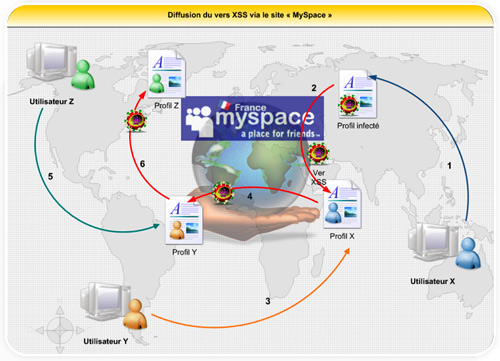
\includegraphics{images/versmyspace.jpg}\\

Comment le pirate a-t-il découvert la faille ?
Il a tout d’abord remarqué que l’insertion de code HTML au sein de son profil était possible. En théorie si l’injection de code HTML est possible, il est également possible d’injecter du code Javascript, c’est à ce niveau que le pirate s’est heurté à un problème. En effet le site Myspace dispose d’une forte restriction en ce qui concerne le terme « javascript » (Ex : <script language= ‘’text/javascript’’) par conséquent l’insertion de ce dernier semblait très délicate. Il a donc trouvé une solution pour contourner ce problème, qui consistait à séparer ce terme en deux parties par retour chariot, ce qui lui a permis ensuite d’exploiter cette faille au maximum.
Ce code JS envoyait discrètement et à l’insu de la victime des requêtes POST et GET via AJAX, la seule condition était que la victime visite le profil de l’utilisateur Samy. Le plus compliqué dans la mise en place de cette faille était la génération de requête http automatique sans la moindre intervention. La victime ne se rendait pas compte que lors de sa visite du profil Samy le navigateur lançait des requêtes http, simplement parce que la validation se faisait automatiquement (très dur à réaliser en JS).
Samy n’a pas été le seul ver à se propager à si grande échelle, il y a eu également le ver « Yammaner » (crée en 2006). Celui-ci a contaminé un grand nombre de serveur web-mail, notamment Yahoo. S’appuyant sur le même principe que Samy, Yammaner avait pour but de voler la liste de contact de la victime. Pour cela cette dernière recevait un email qui une fois ouvert s’envoyait lui-même à tous les contacts de la victime.
		

		\newpage
	
	% Conclusion
	\chapter*{Conclusion} % (fold)
	\addcontentsline{toc}{chapter}{Conclusion}
		Contenu Conclusion

		% Conclusion (end)
		\newpage
	
	% Glossaire
	\renewcommand\glossaryname{Glossaire}
	\addcontentsline{toc}{chapter}{Glossaire}
	\printglossaries
	\newpage
	
	% Bibliographie
	\addcontentsline{toc}{chapter}{Bibliographie}
	\bibliographystyle{plain} % Le style est mis entre crochets. 
	\nocite{*}		
	\bibliography{bibli} % mon fichier de base de données s'appelle bibli.bib
	\newpage
	
	% Liste des figures
	\addcontentsline{toc}{chapter}{Liste des figures}
	\listoffigures
	\newpage
	
	% Annexes	
	\chapter*{Annexes} % (fold)
	\addcontentsline{toc}{chapter}{Annexes}
	
%	\section*{Annexe 1 - Mindmap récapitulative des modules utiles en fonction des besoins}
%	\addcontentsline{toc}{section}{Annexe 1 - Mindmap récapitulative des modules utiles en fonction des besoins}
%		\begin{figure}[!b]
%			\begin{center}		
%				\includegraphics[width=15.5cm]{images/openerp_mindmap.jpg}
%			\end{center}
%		\end{figure}
%	\newpage
	
	% Table des matières
	\addcontentsline{toc}{chapter}{Tables des matières}
	\tableofcontents
	\newpage
\end{document}